\documentclass[11pt,oneside]{article}
\usepackage[T1]{fontenc}
\usepackage[utf8]{inputenc}
%\DeclareUnicodeCharacter{00A0}{ }
\usepackage[adobe-utopia]{mathdesign}

\usepackage{amsmath}
\usepackage[francais]{babel}
\usepackage[dvips]{graphicx}
%\usepackage{here}
\usepackage{framed}
\usepackage[normalem]{ulem}
\usepackage{fancyhdr}
\usepackage{titlesec}
\usepackage{vmargin}

\usepackage{amsmath}
\usepackage{ifthen}
\usepackage{multirow}
\usepackage{multicol} % Portions de texte en colonnes

%\usepackage{xltxtra} % Logo XeLaTeX
%\usepackage{pst-solides3d}
\usepackage{color}
%\usepackage{colortbl}
\usepackage{titletoc} % Pour la mise en forme de la table des matières

%\usepackage[crop=off]{auto-pst-pdf}
%\usepackage{bclogo}


%\usepackage{longtable}
%\usepackage{flafter}%floatants après la référence
%\usepackage{pst-solides3d}
%\usepackage{pstricks}
%\usepackage{minitoc}
%\setcounter{minitocdepth}{4}
%\usepackage{draftcopy}% "Brouillon"
%\usepackage{floatflt}
%\usepackage{psfrag}
%\usepackage{listings} % Permet d'insérer du code de programmation
%\usepackage{lmodern}
%\usepackage[adobe-utopia,uppercase=upright,greeklowercase=upright]{mathdesign}
%\usepackage{minionpro}
%\usepackage{pifont}
%\usepackage{amssymb}
%\usepackage[francais]{varioref}

\setmarginsrb{1.5cm}{1cm}{1cm}{1.5cm}{1cm}{1cm}{1cm}{1cm}

\definecolor{gris25}{gray}{0.75}
\definecolor{bleu}{RGB}{18,33,98}
\definecolor{bleuf}{RGB}{42,94,171}
\definecolor{bleuc}{RGB}{231,239,247}
\definecolor{rougef}{RGB}{185,18,27}
\definecolor{rougec}{RGB}{255,230,231}
\definecolor{vertf}{RGB}{103,126,82}
\definecolor{vertc}{RGB}{220,255,191}
\definecolor{violetf}{RGB}{112,48,160}
\definecolor{violetc}{RGB}{230,224,236}
\definecolor{jaunec}{RGB}{220,255,191}
\usepackage[final]{pdfpages} 
\usepackage[%
    pdftitle={TD Conception},
    pdfauthor={Xavier Pessoles},
    colorlinks=true,
    linkcolor=blue,
    citecolor=magenta]{hyperref}



% \makeatletter \let\ps@plain\ps@empty \makeatother
%% DEBUT DU DOCUMENT
%% =================
\sloppy
\hyphenpenalty 10000

\newcommand{\Pointilles}[1][3]{%
\multido{}{#1}{\makebox[\linewidth]{\dotfill}\\[\parskip]
}}


\begin{document}


\newboolean{prof}
\setboolean{prof}{false}
%------------- En tetes et Pieds de Pages ------------
\pagestyle{fancy}
\renewcommand{\headrulewidth}{0pt}

\fancyhead{}
\fancyhead[L]{%
\begin{minipage}[c]{1.6cm}

\includegraphics[width=2cm]{png/logo_ptsi.png}%
\end{minipage}
\rule{2cm}{.5pt}
}

\fancyhead[C]{\rule{11cm}{.5pt}}

\fancyhead[R]{%
\begin{minipage}[c]{3cm}
\begin{flushright}
\footnotesize{\textit{\textsf{Sciences Industrielles\\ pour l'Ingénieur}}}%
\end{flushright}
\end{minipage}
}

\renewcommand{\footrulewidth}{0.2pt}

\fancyfoot[C]{\footnotesize{\bfseries \thepage}}
\fancyfoot[L]{\footnotesize{2012 -- 2013} \\ X. \textsc{Pessoles}}
\ifthenelse{\boolean{prof}}{%
\fancyfoot[R]{\footnotesize{TD -- CI 4 -- Conception des mécanismes -- P}}
}{%
\fancyfoot[R]{\footnotesize{TD -- CI 4 -- Conception des mécanismes}}
}


%\begin{center}
%\textit{Centre d'intérêt}
%\end{center}


\begin{center}
 \huge\textsc{CI 4 -- Conception des mécanismes}
\end{center}


\begin{center}
 \large\textsc{}
\end{center}
\vspace{.5cm}

\begin{flushright}
\textit{D'après Patrick Beynet \& Al. PTSI, Editions Ellipses.}
\end{flushright}


\subsection*{Motopropulseur de scooter}
L'étude concerne le groupe motopropulseur d'un scooter de $50\; cm^3$, et plus particulièrement son pignon lanceur. 

\begin{center}
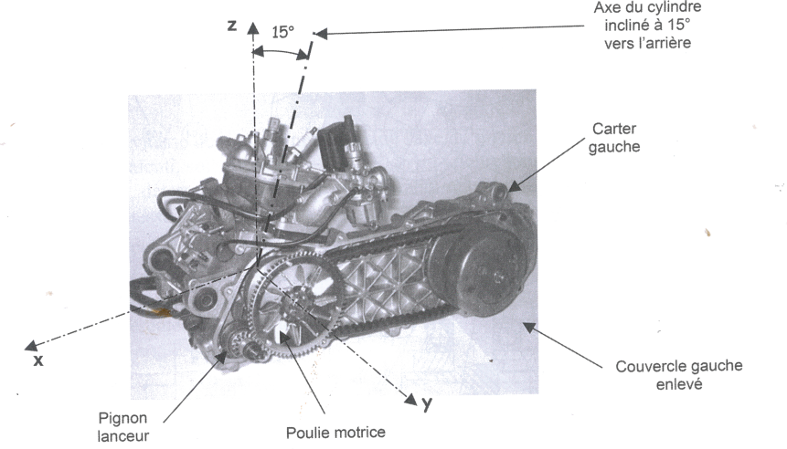
\includegraphics[width=.75\textwidth]{png/fig1}
\end{center}

\begin{center}
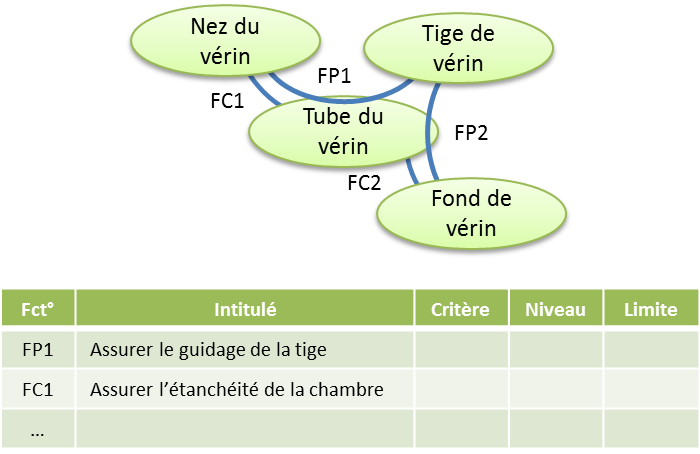
\includegraphics[width=.75\textwidth]{png/fig3}
\end{center}

\begin{center}
\rotatebox{270}{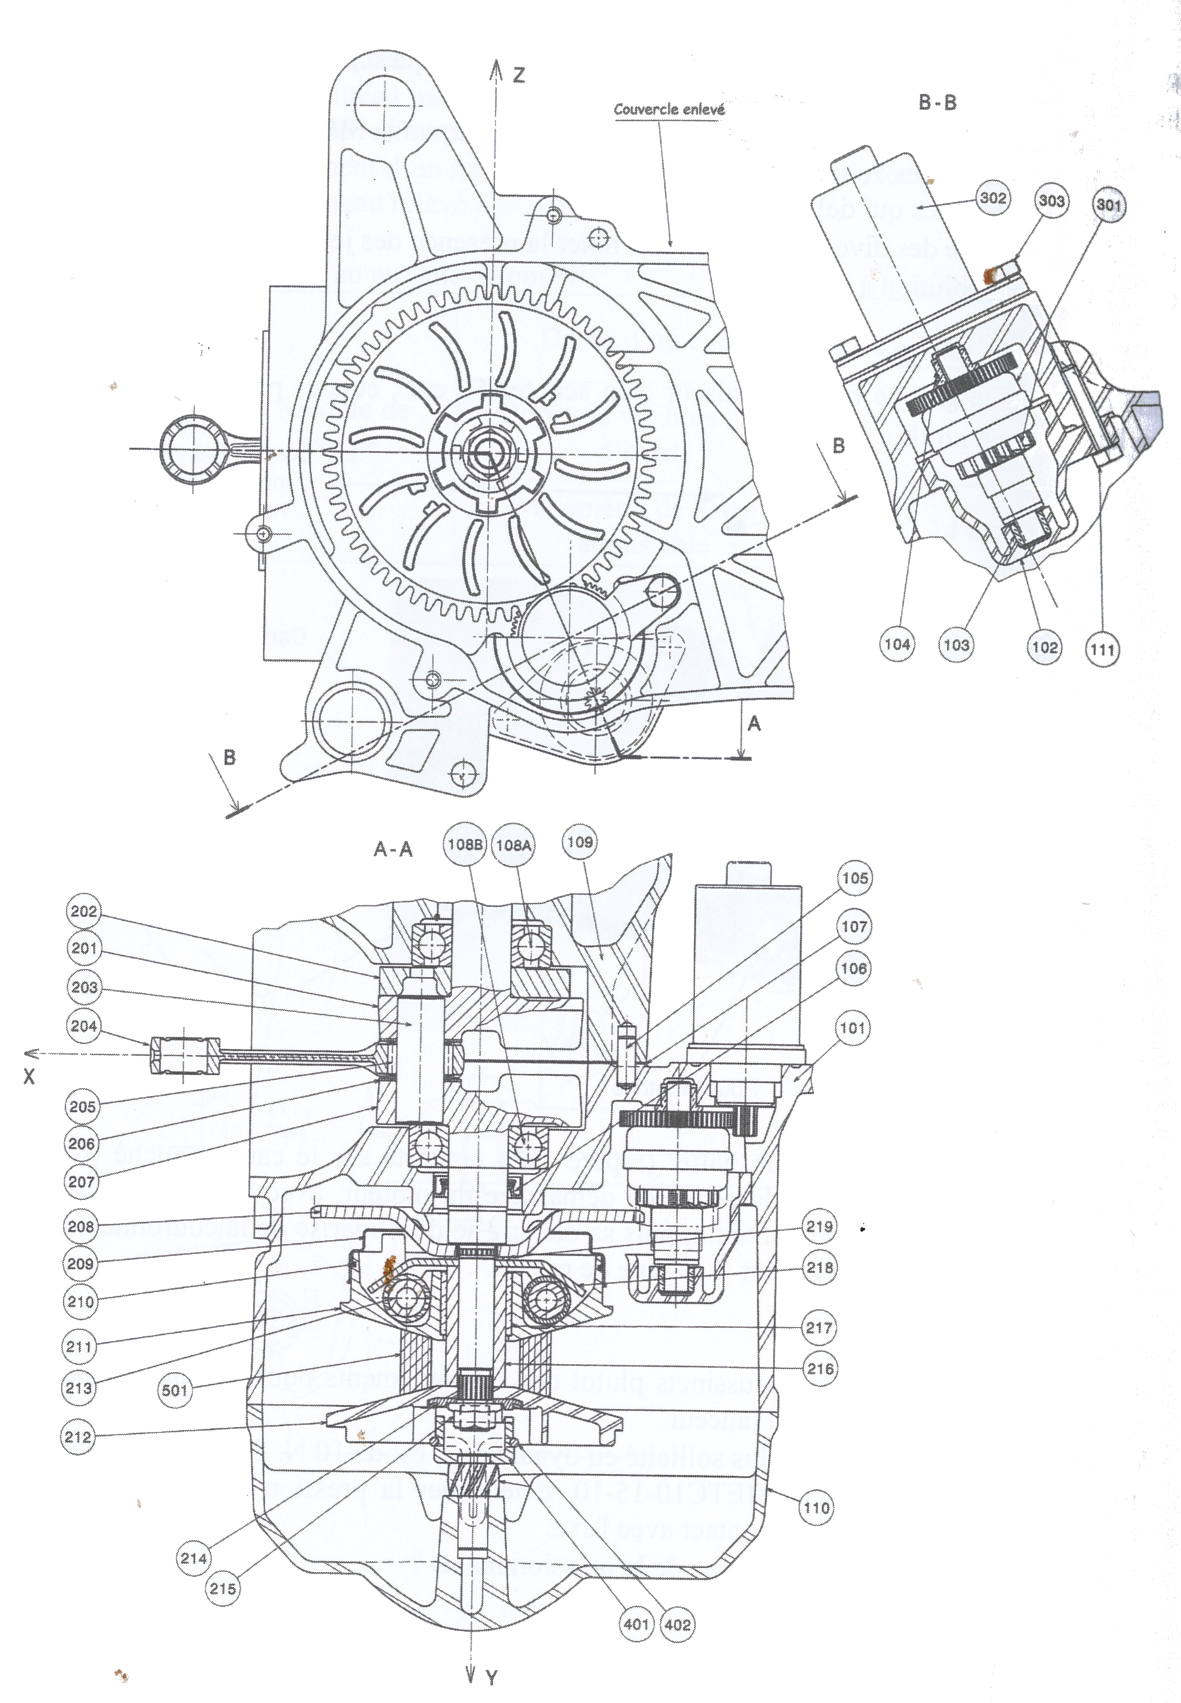
\includegraphics[height=\textwidth]{png/fig2}}
\end{center}




Le pignon lanceur est logé dans un palier (repère 102) rapporté sur le carter gauche (repère 101). Ce pignon engrène pendant la phase de démarrage du moteur avec la couronne dentée (repère 208) pour entraîner le vilebrequin, puis sa denture se désolidarise de la couronne dentée quand le moteur a démarré et a atteint le régime de ralenti. 

\paragraph{}
\textit{Justifier le choix d'emploi de coussinets plutôt que de roulements pour chacun des paliers permettant le guidage du pignon lanceur.}

\paragraph{}
\textit{L'effort radial pour le palier le plus sollicité en dynamique est de 10N. Sachant que le palier a pour référence constructeur METC10-15-10 déterminer la pression supposée uniforme subie par le palier au niveau du contact avec l'axe. }

\paragraph{}
\textit{La pression résiste-t-il au matage (critère de pression maximale) ?}

\paragraph{}
\textit{Sachant que la vitesse de rotation maximale de l'axe du pignon lanceur est atteinte lorsque le moteur est au ralenti, soit une vitesse de rotation du vilebrequin et de la couronne dentée 208 de $1\; 200 tr/min$, déterminer la vitesse de glissement maximum entre l'arbre et le palier lisse. Le critère de vitesse linéaire maximal est-il vérifié ? On donne $Z_{208}=69\; \text{dents}$, $Z_{301}=14 \; \text{dents}$.}

\paragraph{}
\textit{Pourquoi le critère $p\times v$ n'est-il pas essentiel ici ?}


\subsection*{Roue de chariot}
Le dessin ci-dessous représente une roue de chariot qui circule sur un rail incurvé. On admet que l'action transmise du rail sur la roue est définie au point $A$ par le torseur d'action mécanique suivant : 
$$
\torseurc{\mathcal{T}\left(rail \rightarrow roue\right)}{-133}{500}{0}{0}{0}{0}{A,\left(\vect{x},\vect{y},\vect{z}\right)}
$$


\begin{center}
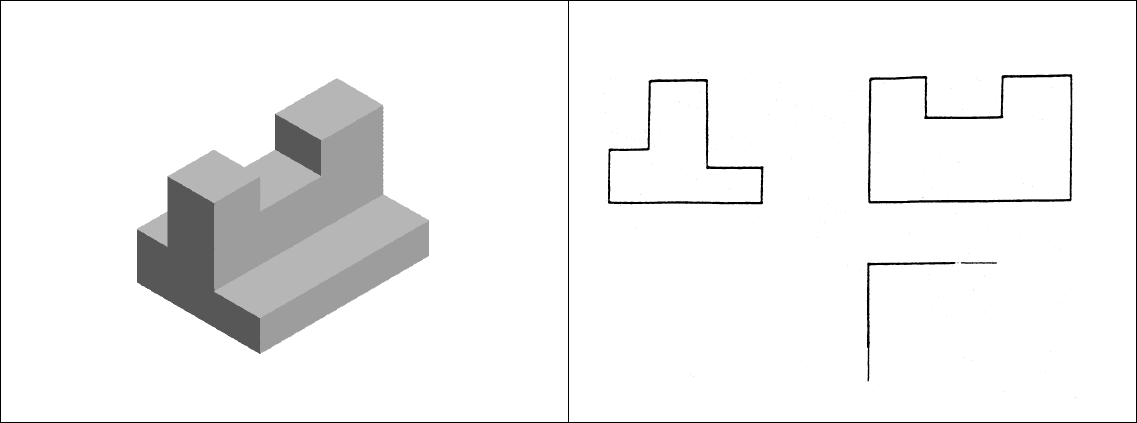
\includegraphics[width=.75\textwidth]{png/fig4}
\end{center}

Le chariot se déplace à une vitesse moyenne de $4\; m/s$, le rayon de la roue vaut $64\; mm$. Compte tenu des actions mécaniques du rail sur la roue, on admettra que le guidage est obtenu par l'association d'une liaison sphère-cylindre en $B$ et d'une liaison rotule en $C$.
%
%Une étude de statique a permis l'obtention des actions du sous ensemble $S_1$ (chariot et coussinets) sur $S_2$ (roue et axe).
%
%$$
%\torseurc{\mathcal{T}_1\left(S_1 \rightarrow S_2\right)}{0}{-1\,000}{0}{0}{0}{0}{B,\left(\vect{x},\vect{y},\vect{z}\right)}
%\quad
%\torseurc{\mathcal{T}_2\left(S_1 \rightarrow S_2\right)}{133}{500}{0}{0}{0}{0}{C,\left(\vect{x},\vect{y},\vect{z}\right)}
%$$

Le diamètre extérieur de l'arbre 7 vaut $35\; mm$. 


\paragraph*{}
\textit{Déterminer les efforts dans chacun des paliers.}

\paragraph*{}
\textit{Vérifier que les coussinets autolubrifiants choisis (longueur : $20\; mm$, diamètre intérieur : $25\; mm$, diamètre extérieur : $32\; mm$, diamètre de collerette :  : $38\; mm$) sont pertinents par rapport aux critères de pression maxi, vitesse maxi et produit $p\times v$ (critère énergétique). On admettra des répartitions uniformes pour les différents champs de pression.}

Le constructeur fournit les caractéristiques suivantes pour les coussinets autolubrifiants en bronze fritté : 
$p_{maxi} = 10\; MPa$, $v_{maxi} = 6m/s$; $\left(p\times v \right)_{maxi}=2\;MPa \cdot m/s$.


\paragraph*{}
\textit{Déterminer la longueur de la clavette. La pression de matage admissible est de $40\; MPa$.}
\begin{center}
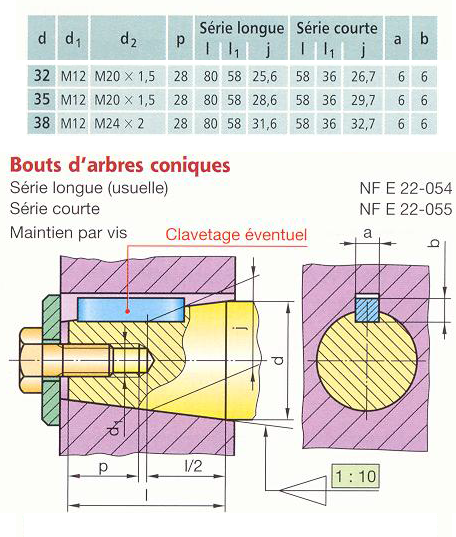
\includegraphics[width=.6\textwidth]{png/fig5}
\end{center}


\end{document}